\documentclass{beamer}
\usepackage[utf8]{inputenc}
\usepackage[T1]{fontenc}
\usepackage{color}
\usepackage{listings}
\usepackage{booktabs}
\usepackage{pdfpages}
\usepackage{mathtools}
\usepackage{enumerate}
\usepackage{multirow,tabularx}
\usepackage{booktabs}
\usepackage{pdfpages}
\usepackage{proof}
\usepackage{cancel}
\usepackage{chronology}
\usepackage{graphicx}
\usepackage{ulem}
\usepackage{amsmath}
\usepackage{amssymb}

\title{Knowledge Representation \& Ontology}
\subtitle{MSc Bioinformatics \\ Slides: http://lokero.xyz/msc.pdf}
\author{Luke Slater (lxs511@bham.ac.uk)}
\institute{Centre for Computational Biology \\ University of Birmingham}
\date{28/11/2018}

\begin{document}

\frame{\titlepage}

\begin{frame}
\frametitle{Objectives}

\begin{itemize}
  \item Just Semantics
  \item How do we express and represent knowledge?
  \item How can computers express and represent knowledge?
  \begin{itemize} 
    \item HTML: a degenerate form of XML
    \item XML: a degenerate form of RDF
    \item The Resource Description Framework (RDF)
  \end{itemize}
  \item Ontologies
  \begin{itemize} 
    \item What are they?
    \item What do they know? Do they know things? Let's find out!
    \item Differences between ontologies \& databases
  \end{itemize}
  \item Afternoon: Practical
\end{itemize}
\end{frame}

\begin{frame}
\frametitle{Moving from Information to Knowledge and Wisdom}
\begin{columns}
\column{0.5\textwidth}

\centering{
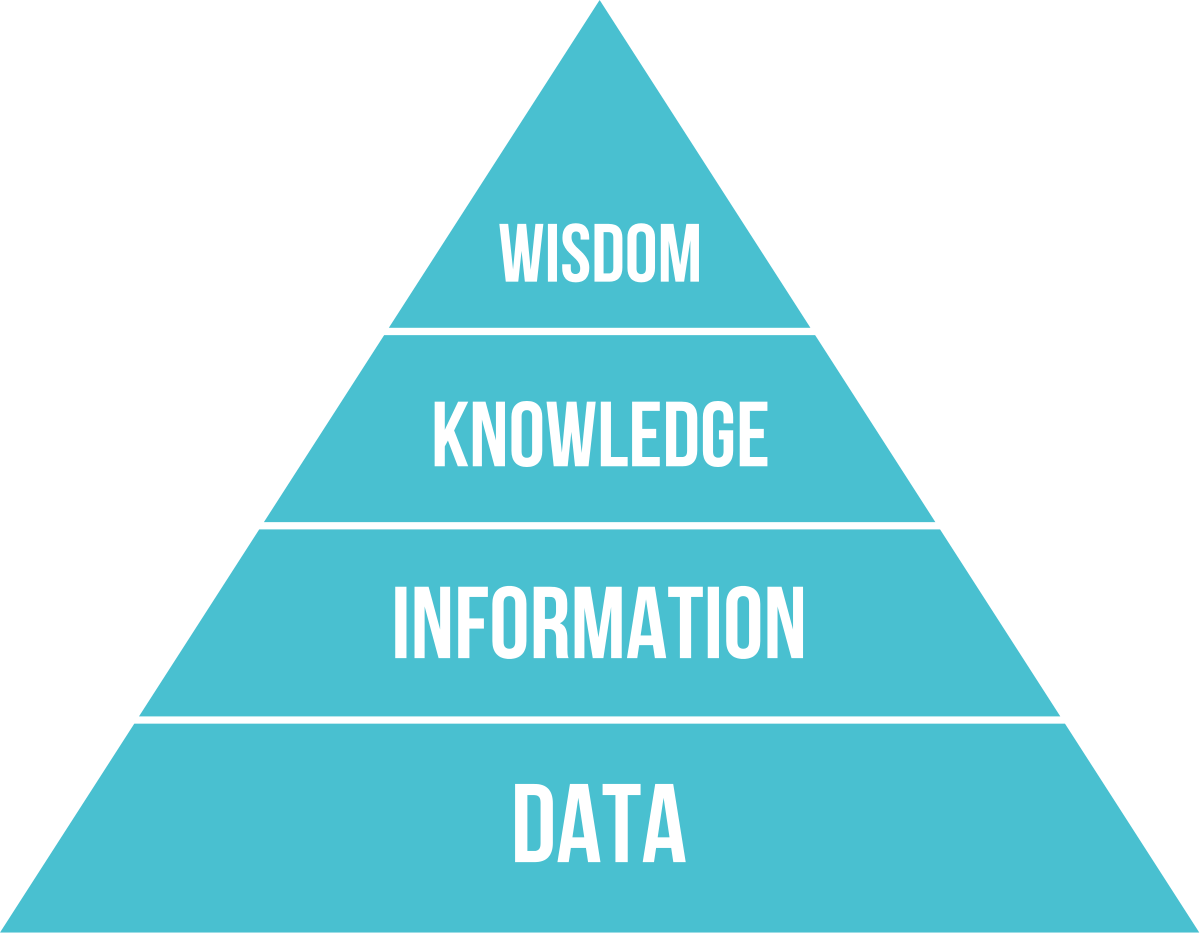
\includegraphics[width=\textwidth]{pyramid.png}
}

\column{0.5\textwidth}

\begin{itemize}
  \item We've previously spoken about how to take some data and represent it as
  information and then to use it as knowledge.
  \item Now, we will consider how we can move, computationally, from information
  to knowledge and finally to wisdom.
\end{itemize}

\end{columns}

\end{frame}

\begin{frame}
\frametitle{Digression on Epistemology}
\begin{itemize}
  \item What does it mean to know something? What is knowledge? Even for humans, it is an unsolved
  problem.
  \item For a long time, Justified True Belief was regarded as an adequate
  solution for the question of what it means to know something. You can be said
  to know something if your assertion meets the following conditions:
  \begin{enumerate}
    \item You \emph{believe} the proposition is true.
    \item Your belief is somehow \emph{justified} (you have a reason to believe
    it).
    \item The proposition itself is \emph{true}.
  \end{enumerate}
  \item In 1963, Edmund Gettier released a mere 3-page paper defeating this notion by
  introducing the Gettier Problem...
  \item Nevertheless, we persist with this general idea of knowledge, for the
  most part.
\end{itemize}
\end{frame}

\begin{frame}
\frametitle{Definition on Wisdom}

\large{Likely as many definitions as there are people who know the word, but in
this case we mean: the ability to think and act using \emph{knowledge}.}

\end{frame}

\begin{frame}
\frametitle{Symbols: Treachery of Images}

\centering{
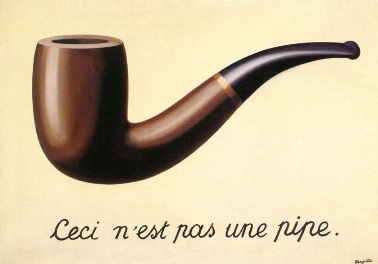
\includegraphics[width=\textwidth]{prop.jpg}
}
\end{frame}

\begin{frame}
\frametitle{Symbols and their Meanings}

\begin{itemize}
  \item This treachery lies not only in what might be called a picture, but also
  in words. For words are just another kind of image, or symbol.
  \item And so, what does it actually mean to be that which we refer when we say
  \emph{pipe}?
  \item And how does the symbol \emph{pipe} come to carry this meaning?
  \item Do these language symbols somehow
  directly correspond to reality (as in a picture), or are they very human mental
  constructs pointing vaguely at reality? (former: see Wittgenstein, latter: see
  later Wittgenstein).
\end{itemize}
\end{frame}

\begin{frame}
\frametitle{Consensus Meaning}

\begin{itemize}
  \item These symbols are imbued with meaning by a complex cultural process of
  consensus, which is in a state of constant flux and ambiguity.
  \item We further describe both particular objects (you) and classes of objects
  (Human) with complicated syntactic forms, from which meaning is also derived
  in a cognitive process fraught with constant flux and ambiguity.
  \item Things are complicated further when we consider what might be said 
  about an abstract noun, such as peace, green, or disco.
\end{itemize}
\end{frame}

\begin{frame}
\frametitle{The Syntactic Web}
\begin{itemize}
  \item We all know the syntactic web: the sum of human knowledge presented in natural 
  language, and intended for human interaction.
  \item As such, meaning is derived and agreed by offline consensus.
  \item Examples: Wikipedia, BBC news, Facebook, most websites as you know them.
\end{itemize}
\end{frame}

\begin{frame}
\frametitle{Computers:}

\begin{itemize}
  \item Can count higher than you
  \item Needs to be a supercomputer to identify a dog
\end{itemize}
\centering{
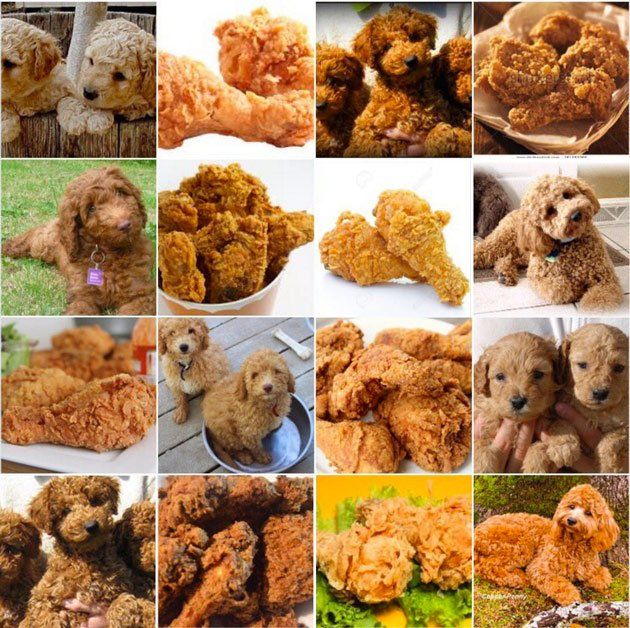
\includegraphics[width=0.6\textwidth]{dog.jpg}
}
\end{frame}

\begin{frame}
\frametitle{Natural Language Processing}

\centering{
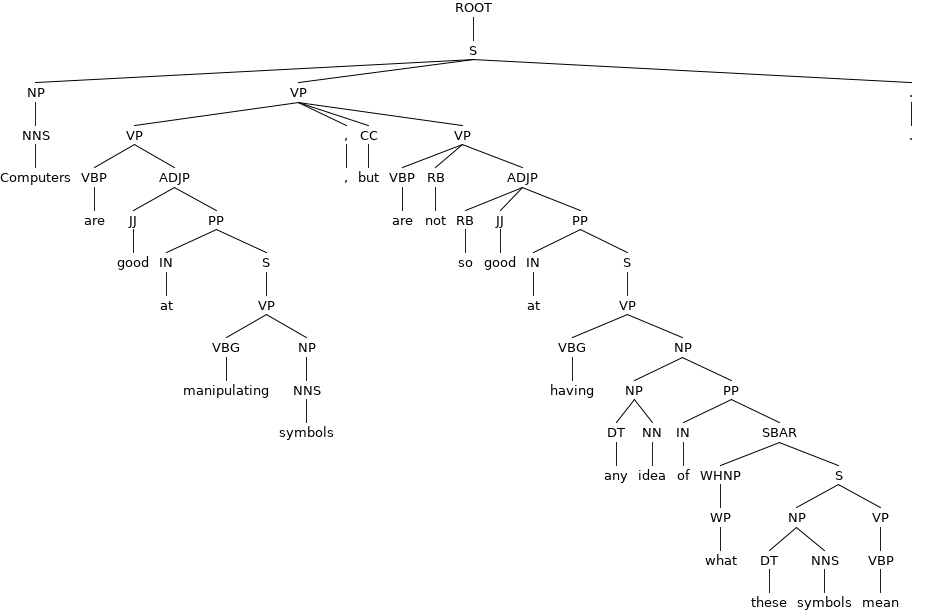
\includegraphics[width=\textwidth]{nlp.png}
}
\end{frame}

\begin{frame}
\frametitle{Limitations of Classical Natural Language Processing}

\begin{itemize}
\item Consider the sentence "I made her fish," which has at least five potential
meanings (double for plurality!):

\begin{enumerate}
  \item I cooked a fish for her.
  \item I cooked a fish belonging to her.
  \item I created the fish she owns.
  \item I forced her to go fishing.
  \item I made her into the Platonic ideal Fish.
\end{enumerate}

\item All problems in NLP may be reduced to the question of ambiguity - and it is
\emph{everywhere}; in human language, symbolic equivalence is not equivalent to semantic equivalence.

\end{itemize}
\begin{minipage}[t][.2\textheight]{\textwidth}
\tiny{Example inspired by "Speech and Natural Language
Processing" 2nd ed by Daniel
Jurafsky \& James H. Martin.}
\vfill
\end{minipage}
\end{frame}

\begin{frame}
\frametitle{The Limitation: Ambiguity and Meaning}

\begin{itemize}
  \item Computers are good at manipulating symbols, but are not so good at
  having any idea of what these symbols mean - their semantics.
  \item Furthermore, they struggle to translate symbols from ambiguous (read:
  human) languages into definite symbols to manipulate.
\end{itemize}
\end{frame}

\begin{frame}
\frametitle{The Problem}

\begin{itemize}
  \item How do we make a computer \emph{understand} the objects that we're describing,
  and the relationships between them?
  \item How can we make a computer \emph{know} something?
  \item How can we gain wisdom from the knowledge we give a computer?
  \item Requirements:
  \begin{enumerate}
    \item To be able to describe and to predicate upon \emph{particular}
    entities. For example: \emph{this gibbon is very angry}, or \emph{this tomato is
    mouldy}.
    \item To be able to define the \emph{kinds of} entities which may exist, and
    the relationships they may have between them. For example: \emph{a hand may have
    fingers}, or \emph{a parent must have a child}.
  \end{enumerate}
\end{itemize}
\end{frame}

\begin{frame}
\frametitle{Separating the entity and the instance}
 \begin{itemize}
  \item This separation of the class and the particular is along the lines of
  the Plato's Theory of Forms, or more generally Idealism: that particular
  objects (a chair) are partaking in a pure form which idealises and represents
  the most accurate reality of that object (The Chair or Chairness).
  \item This is one solution to the metaphysical problem of Universals.
  \item While rife with philosophical problems (much like any alternative
  theory), it happens to be extremely useful to us: computer scientists may
  notice a strong correlate when considering Object Orientated Programming:
  Classes and Instances.
\end{itemize}
\end{frame}

\begin{frame}
\frametitle{The Semantic Web}

\begin{itemize}
  \item Utilises the infrastructure of the world wide web as a data
  communication methodology.
  \item Instead of only presenting data: link, interpret, and analyse data.
  \item In the consumer sphere this forms the basis for the 'Internet of
  Things.' 
\end{itemize}
\end{frame}

\begin{frame}
\frametitle{Describing instances}

\begin{columns}
\column{0.5\textwidth}


\includegraphics[width=\textwidth]{html.jpg}

\column{0.5\textwidth}

Almost accidentally, the means by which we could develop a semantic
framework for knowledge representation was already in heavy use throughout the
world wide web.

\end{columns}
\end{frame}

\begin{frame}
\frametitle{HTML}
Web pages are created in HyperText Markup Language (HTML)
\begin{columns}

\column{0.6\textwidth}

\lstinputlisting[language=HTML]{example.html}

\column{0.4\textwidth}

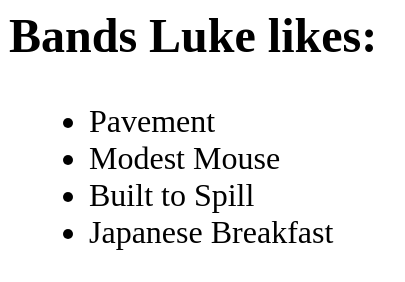
\includegraphics[width=\textwidth]{list.png}

\end{columns}
\end{frame}

\begin{frame}
\frametitle{Natural Language Inference}

\begin{itemize}

\item The assertions we can infer from this text are numerous:

\begin{enumerate}
  \item A person exists.
  \item A person is named Luke.
  \item There is at least one person.
  \item The person Luke likes some bands.
  \item At least four bands exist.
  \item Some people like bands.
  \item Pavement, Modest Mouse, Built to Spill, Japanese Breakfast are bands.
  \item Luke stands in a relationship of likes with all these bands.
  \item Some bands are liked.
  \item At least one person likes Pavement, Modest Mouse, Built to Spill, and
  Japanese Breakfast.
\end{enumerate}

\end{itemize}

\end{frame}

\begin{frame}
\frametitle{HTML: A Degenerate Form of XML}

\begin{itemize}
  \item HTML was later generalised, to create the eXtensible Markup Language
  (XML), without a focus on describing how a document should be rendered
  visually.
  \item This is a more general markup language, which can organise and "mark up" 
  or extend any kind of textual data with any additional information.
\end{itemize}

\end{frame}

\begin{frame}
\frametitle{RDF: An Exhilirate Form of XML}

\begin{itemize}
  \item A method of representing structured data for the semantic web.
  \item Used heavily within science for experimental results, datasets and
  various open data, particularly in the biological and biomedical domains.
\end{itemize}

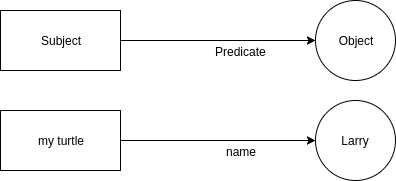
\includegraphics[width=\textwidth]{two.png}
\end{frame}

\begin{frame}
\frametitle{RDF: Semantic Networks}
\centering{
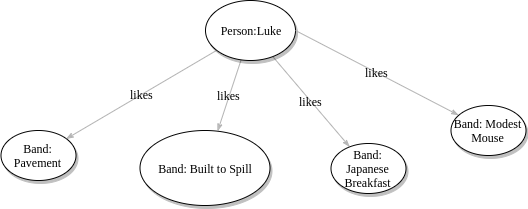
\includegraphics[width=\textwidth]{bands.png}
}
\end{frame}

\begin{frame}
\frametitle{Wikipedia vs DBPedia}
\begin{columns}

\column{0.5\textwidth}

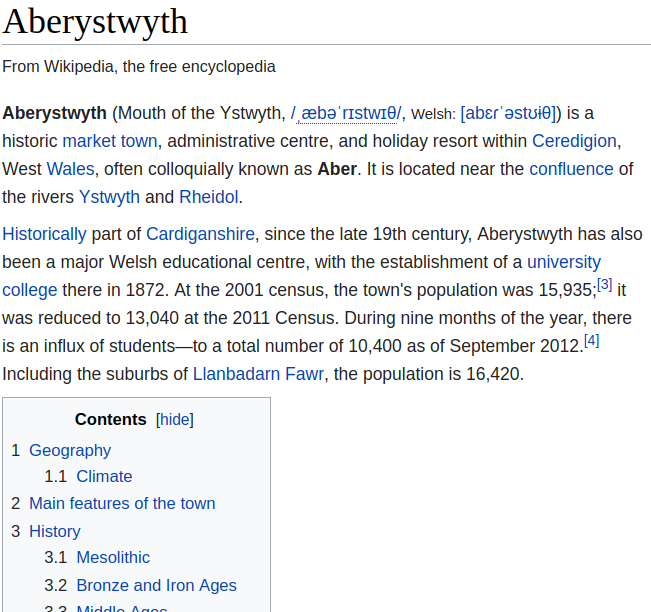
\includegraphics[width=\textwidth]{aberwiki.png}

\column{0.5\textwidth}

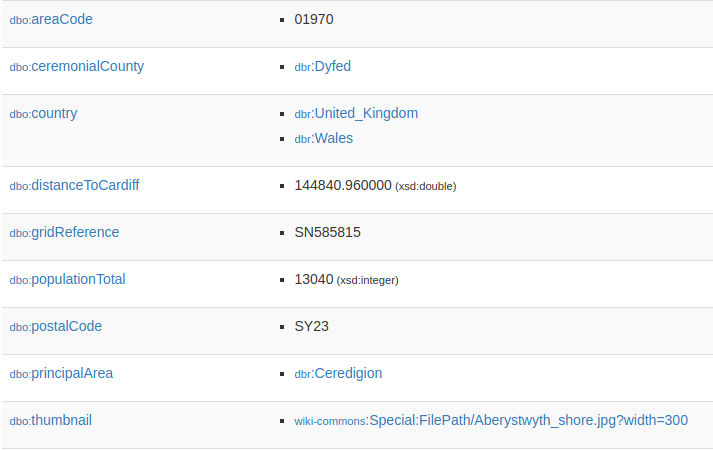
\includegraphics[width=\textwidth]{aberpedia.png}

\end{columns}
\end{frame}

\begin{frame}
\frametitle{What is an ontology, anyway?}

\centering{

\includegraphics[width=0.7\textwidth]{questionowl.png}
}

\end{frame}

\begin{frame}
\frametitle{Ontology: Describing the objects} \begin{itemize}
  \item Ontologies categorise, define and relate the kinds of things in a domain.
  \item Easily thought of as the 'schema' for the data represented by RDF (and
  in any other format).
  \item Exact definitions differ, but most ontologies share four main features:
  \begin{enumerate}
    \item Classes and relations.
    \item Domain vocabulary.
    \item Metadata and descriptions.
    \item Axioms and formal definitions.
  \end{enumerate}
\end{itemize}
\end{frame}

\begin{frame}
\frametitle{Ontology: Classes (and relations)}
\begin{itemize}
  \item A class is a category of things which can exist within a
  particular world, defined by the necessary and sufficient conditions for a
  thing to exist within that category (intensional definition).
  \item Each distinct class has its own IRI (Internationalised Resource
  Identifier), but may share labels, descriptions, or any other information with
  other classes.
  \item This does not necessarily make them semantically equivalent!
  \item e.g. HP:0002457 and MP:0000436 both have the label 'abnormal head
  movements'
\end{itemize}
\end{frame}

\begin{frame}
\frametitle{Ontology: (Classes and) relations}
\begin{itemize}
  \item Also concerned with the relationships between things. A fundamental
  relationship between classes is the is-a relationship.
  \item All ontologies start with the root class \emph{Thing}, and all other 
  classes in the ontology stand in a transitive subclass relationship to it.
  \item In this way, they form, at a most basic level, a taxonomy of
  categorisation for a particular universe of interest.
  \item Other common relationships are: part-of, inheres-in, caused-by,
  regulates.
  \item Many relationships carry deeply argued issues and side-effects: fingers!
\end{itemize}
\end{frame}

\begin{frame}
\frametitle{Ontology: Domain Vocabulary}

\begin{itemize}
  \item Structured vocabulary for a domain
  \item Usually provided in the form of short 'labels' for each class (can have
  multiple)
  \item Provision for translated terms for classes
  \item Synonyms; the same category of things in a different context
  \item Together with the structure of the ontology, we gain a large and
  well-organised set of relevant terms for our domain
  \item Reduces ambiguity and misunderstanding in the conceptualisation for a
  domain
\end{itemize}
\end{frame}

\begin{frame}
\frametitle{Ontology: Domain Vocabulary}
\centering{
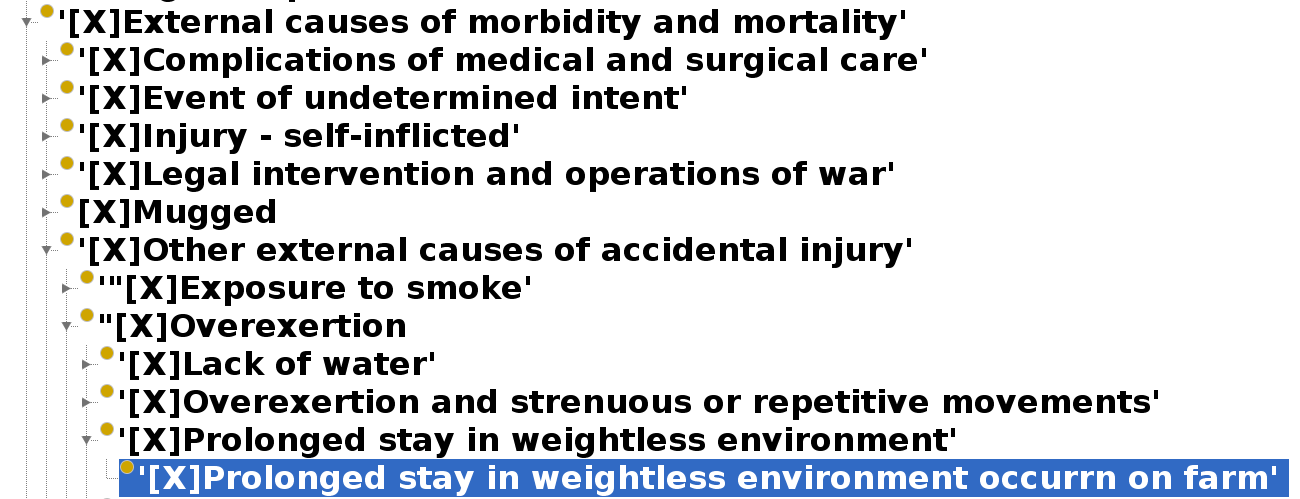
\includegraphics[width=\textwidth]{read.jpg}
}
\end{frame}

\begin{frame}
\frametitle{Ontology: Metadata and Descriptions}

\begin{itemize}
  \item Descriptions, usually provided using the genus-differentia method.
  \begin{description}
    \item[temporal pattern] The speed at which disease
    manifestations appear and develop.
    \item[insidious onset] \textcolor{red}{Gradual, very slow}
    \textcolor{blue}{onset of disease manifestations}
  \end{description}
  \item Database cross-links, providing an assurance of semantic equivalence to
  data about an entity from an external source.
\end{itemize}
\end{frame}

\begin{frame}
\frametitle{Ontology: Axioms and Formal Definitions}

\begin{itemize}
  \item The formal aspect of ontologies, axiomatic expression of meaning.
  \item Example: hypertension defined as \textcolor{green}{has part}
  \textcolor{red}{some} ((\textcolor{blue}{blood} \textcolor{red}{and}
  (\textcolor{green}{part-of} \textcolor{red}{some} \textcolor{blue}{arterial
  system})) \textcolor{red}{and} (\textcolor{green}{has-quality}
  \textcolor{red}{some}
  ((\textcolor{blue}{increased pressure} \textcolor{red}{and}
  (\textcolor{green}{has-modifier} \textcolor{red}{some}
  \textcolor{blue}{chronic})) and (\textcolor{green}{has-modifier}
  \textcolor{red}{some}
  \textcolor{blue}{abnormal}))))
  \item Enable semantic analysis and (ostensibly) cross-species integration of
  knowledge.
\end{itemize}
\end{frame}

\begin{frame}
\frametitle{Ontology Reasoning}

\begin{itemize}
  \item Reasoning is the use of a classifier to evaluate all logical consequences
  of the explicit statements in an ontology.
  \item This allows us to infer new knowledge, and evaluate the consistency of our
  logical model (and can tell us why in the case of inconsistency).
  \item There are many different reasoners, which use slightly different methods
  and support different subsets of description logic (they are often said to have
  different levels of ‘expressivity’).
\end{itemize}
\end{frame}

\begin{frame}
\frametitle{How do ontologies differ from databases?}

 \begin{table}[ht]
    \centering
    \begin{tabular}{|l|l|}
      Database & OWL Ontology \\
      \hline
      Closed World Assumption & Open World Assumption \\
      Unique Name Assumption & No UNA \\
      Schema constraints data structure %, defining legal states of
                                %the database 
               & Axioms behave like inference rules\\\hline
    \end{tabular}
\end{table}
\end{frame}

\begin{frame}
\frametitle{Web Ontology Language (OWL)}

\begin{itemize}
  \item Poor acronym, reference to Winnie the Pooh.
  \item Based on description logics, a fragment of first order logic.
  \item A set of language specifications based on description logics.
  \begin{description}
    \item[Full] Every construct in OWL is available. Fully undecidable to
    reason. Cardinality restrictions, domain, range, and value restraints.
    \item[EL] Subset of OWL which is guaranteed to be classifiable in polynomial
    time. Only way to reach inconsistency is through disjointness.
    \item[RL] A subset which mirrors the features of relational databases.
  \end{description}
  \item Less expressive reasoners can simply ignore the more expressive content
  within ontologies.
\end{itemize}
\end{frame}

\begin{frame}
  \begin{itemize}
  \item {\tt X SubClassOf: Y}: $X \xrightarrow{\text{is-a}} Y$
  \item {\tt X SubClassOf: part-of some Y}: $X \xrightarrow{\text{part-of}} Y$
  \item {\tt X SubClassOf: regulates some Y}: $X \xrightarrow{\text{regulates}} Y$
  \item {\tt X DisjointWith: Y}: $X \xleftrightarrow{\text{disjoint}} Y$
  \item {\tt X EquivalentTo: Y}: $X \xleftrightarrow{\equiv} Y$, $\{X,Y\}$
\end{itemize}
\end{frame}

\begin{frame}
  \frametitle{OWL Syntax}
  \begin{itemize}
  \item originally an extension of RDF and RDF Schema
  \item Several different (mostly) syntaxes
  \end{itemize}
  Consider the axiom $Parent \equiv Human \sqcap \exists hasChild.\top$
\end{frame}

\begin{frame}[fragile]
  \frametitle{Functional Syntax}
\begin{verbatim}
EquivalentClasses(:Parent 
  ObjectSomeValuesFrom(:hasChild owl:Thing))
\end{verbatim}
\end{frame}

\begin{frame}[fragile]
  \frametitle{RDF/XML Syntax}
{\tiny
\begin{verbatim}
    <owl:Class rdf:about="http://example.com/demo-ontology.owl#Parent">
        <owl:equivalentClass>
            <owl:Restriction>
                <owl:onProperty rdf:resource="http://example.com/demo-ontology.owl#hasChild"/>
                <owl:someValuesFrom rdf:resource="&owl;Thing"/>
            </owl:Restriction>
        </owl:equivalentClass>
    </owl:Class>
\end{verbatim}
}
\end{frame}

\begin{frame}[fragile]
  \frametitle{RDF Turtle Syntax}
{\tiny
\begin{verbatim}
:Parent rdf:type owl:Class ;
        
        owl:equivalentClass [ rdf:type owl:Restriction ;
                              owl:onProperty :hasChild ;
                              owl:someValuesFrom owl:Thing
                            ] .
\end{verbatim}
}
\end{frame}

\begin{frame}[fragile]
  \frametitle{OWL/XML Syntax}
{\tiny
\begin{verbatim}
    <EquivalentClasses>
        <Class IRI="#Parent"/>
        <ObjectSomeValuesFrom>
            <ObjectProperty IRI="#hasChild"/>
            <Class abbreviatedIRI="owl:Thing"/>
        </ObjectSomeValuesFrom>
    </EquivalentClasses>
\end{verbatim}
}
\end{frame}

\begin{frame}[fragile]
  \frametitle{Manchester OWL Syntax}
{\tiny
\begin{verbatim}
Class: Parent
    EquivalentTo: 
        hasChild some owl:Thing
\end{verbatim}
}
\end{frame}

\begin{frame}
  \frametitle{Manchester OWL Syntax}
  \begin{table}[ht]
    \centering
    \begin{tabular}{|l|l|l|}
      DL Syntax & Manchester Syntax & Example \\
      \hline
      $C \sqcap D$ & C and D & Human and Male \\
      $C \sqcup D$ & C or D & Male or Female \\
      $\neg C$ & not C & not Male \\
      $\exists R.C$ & R some C & hasChild some Human \\
      $\forall R.C$ & R only C & hasChild only Human \\
      $(\geq n R.C)$ & R min n C & hasChild min 1 Human \\
      $(\leq n R.C)$ & R max n C & hasChild max 1 Human \\
      $(= n R.C)$ & R exactly n C & hasChild exactly 1 Human \\
      $\{a\} \sqcup \{b\} \sqcup ...$ & \{a b ...\} & \{John Robert
                                                      Mary\} \\
      \hline
    \end{tabular}
  \end{table}
\end{frame}


\begin{frame}
\frametitle{Basic Inference Example}

\begin{enumerate}
  \item All meat comes from animals. (\textcolor{blue}{meat}
  \textcolor{red}{comes-from} \textcolor{blue}{animal})
  \item All beef is meat. (\textcolor{blue}{beef} \textcolor{red}{is-a}
  \textcolor{blue}{meat})
  \item Therefore, all beef comes from animals.
\end{enumerate}
A simple subsumptive relationship, if the first two statements are true (note: our
ontology isn't concerned with the truth of the statements), then the conclusion
is necessarily true. So, our reasoner will add this logical statement to the
ontology (\textcolor{blue}{beef} \textcolor{red}{comes-from} \textcolor{blue}{animal})
\end{frame}

\begin{frame}
\frametitle{Basic Inconsistency Example}

\begin{itemize}
\item \textcolor{blue}{Reptile} \textcolor{red}{is-a NOT} \textcolor{blue}{Mammal}
\item \textcolor{blue}{Person} \textcolor{red}{is-a} \textcolor{blue}{Mammal}
\item \textcolor{blue}{Turtle} \textcolor{red}{is-a} \textcolor{blue}{Reptile}
\item \textcolor{blue}{Turtle} \textcolor{red}{is-a} \textcolor{blue}{Person}
\end{itemize}

Because a turtle is necessarily a reptile, and a reptile is necessarily not a
mammal, a turtle cannot be both a reptile and a person. 
\end{frame}

\begin{frame}
\large{Questions}
\end{frame}

\end{document}
